%#! To typeset this document:
% -----
% First you should get ``pxjahyper.sty'' from CTAN (http://www.ctan.org/pkg/pxjahyper),
% in order to prevent Japanese characters in bookmarks of PDF files from corruption.
% Then typeset:
%  1.  platex usage.tex
%  2.  pdflatex -shell-escape ChemFigFile.tex
%  3.  platex usage.tex (for three times: needed to get cross-references correct)
%  4.  dvipdfmx usage.tex
% Some things to note:
% - ``platex'' is NOT ``pdflatex''!
%   (platex is an engine customized for typesetting Japanese LaTeX documents properly.)
% - ``extractbb'' must be set as shell_escape_commands.
%   (see http://oku.edu.mie-u.ac.jp/~okumura/texwiki/?PDF%E3%81%AE%E4%BD%9C%E3%82%8A%E6%96%B9#rf074b4b for detail)
% -----
% Other requirements (obabel and inkscape) are described in this document itself. See PDF version.
%
%% 
%% This document describes the usage of `chemobabel.sty',
%% a LaTeX package for generating chemical structural formulas using Open Babel and Inkscape.
%% 
%% Copyright 2014 Acetaminophen (Hironobu YAMASHITA)
%%   Email  :     h.y.acetaminophen[a t]gmail.com
%%   GitHub :     https://github.com/aminophen
%%   Blog   :     http://acetaminophen.hatenablog.com/
%% 
%
\documentclass[12pt]{jsarticle}
\usepackage[left=20mm, right=20mm, top=20mm, bottom=20mm]{geometry}
\usepackage[dvipdfmx]{graphicx}
\usepackage[english]{babel}
\usepackage[extract]{chemobabel}
\usepackage[dvipdfmx,bookmarksnumbered=true,%pdfborder={0 0 0},setpagesize=false,%
 pdftitle={chemobabel.sty},pdfauthor={Hironobu Yamashita (Acetaminophen)},pdfsubject={TeX & LaTeX Advent Calendar 2014},%
 pdfkeywords={chemistry,open babel,chemdraw,smiles}]{hyperref}
\usepackage{pxjahyper}
\usepackage{footnotebackref}
% --- Change the style of captions (Japanese jsarticle style => English style) ---
\makeatletter
\long\def\@makecaption#1#2{
\vskip\abovecaptionskip
\sbox\@tempboxa{#1: #2}
\global\@minipagefalse
\hbox to\hsize{\hfil\box\@tempboxa\hfil}
\vskip\belowcaptionskip
}
\makeatother
% --- XyMTeX logo definition ---
\newcount\TestCount
\def\XyM{\ifnum\fam=-1\relax\fam=0\relax\fi\TestCount=\fam%
X\kern-.30em\smash{\raise.50ex\hbox{$\fam\TestCount\Upsilon$}}%
\kern-.30em{M}}
\def\XyMTeX{\XyM\kern-.1em\TeX}
% ------
\title{\textsf{chemobabel.sty} \\[1ex] \normalsize --- Chemical Strucrures from MDL Molfiles, ChemDraw Files or SMILES Notations --- \\ 化学構造式を MOL ファイルや ChemDraw ファイル、SMILES 表記法から自動生成}
\author{Acetaminophen (アセトアミノフェン)}
\begin{document}
\renewcommand{\figurename}{Fig.\,}
\pagenumbering{roman}
\maketitle

This document describes the usage of \textsf{chemobabel.sty} and accompanying macros, a package bundle for \textbf{generating chemical structural formulas} to be inserted in your {\LaTeX} documents.
The formulas can be generated \textbf{from many kinds of chemical data formats}, including MDL Molfiles, ChemDraw files and even from SMILES notations, with the help of Open Babel and Inkscape.
This document is written in both English and Japanese.
The formulas below are generated using this method. \\

この文書では、\LaTeX 文書中に挿入する\textbf{化学構造式を生成}するパッケージである \textsf{chemobabel.sty} と同梱リソースの使い方を説明します。
構造式は Open Babel と Inkscape の機能を利用することにより、MDL Molfile, ChemDraw ファイル、さらには SMILES 表記法を含む\textbf{さまざまな化学データ形式から生成}することができます。
説明は英語と日本語の両方で書かれています。
以下の構造式はこの方法によって出力されたものです。 \\

\begin{figure}[ht]
  \centering
  \chemobabel[scale=0.5]{draw/Firefly luciferin.mol}{}
  \chemobabel[scale=0.27]{draw/Brevetoxin A.mol}{}
  \caption{Firefly luciferin \& Brevetoxin A (from MDL Molfiles)}
\end{figure}

\begin{figure}[ht]
  \centering
  \chemobabel[scale=0.5]{draw/ATP.cdx}{}
  \chemobabel[scale=0.5]{draw/Glucose.cdx}{}
  \caption{ATP (Adenosine triphosphate) \& Glucose (from ChemDraw files)}
\end{figure}

\begin{figure}[ht]
  \centering
  \smilesobabel[scale=0.6]{CCO}{}
  \smilesobabel[scale=0.6]{CC(C(=O)O)N}{}
  \smilesobabel[scale=0.5]{C1[C@H](C)C[C@@H](O)C1}{}
  \caption{Ethanol, Alanine \& (1\textit{S},3\textit{S})-3-Methylcyclopentanol (from SMILES notations)}
\end{figure}

\begin{figure}[ht]
  \centering
  \smilesobabel[scale=0.5]{CC(=O)Nc1ccc(cc1)O}{}
  \smilesobabel[scale=0.5]{C([C@@H]1[C@H]([C@@H]([C@H]([C@H](O1)O)O)O)O)O}{}
  \caption{Acetaminophen (Paracetamol) \& $\alpha$-\textsc{d}-Glucose (from SMILES notations)}
\end{figure}

\clearpage
\setcounter{tocdepth}{3}
\tableofcontents

\clearpage
\pagenumbering{arabic}

\section{Introduction (はじめに)}

\subsection{Motivation for Development (開発の動機)}

\subsubsection{English}

As you already know, {\LaTeX} is being used all over the world.
However, when it comes to drawing chemical strucutral formulas, ways of inserting formulas into {\LaTeX} documents are very limited.
I think it is mainly due to lack of both reliable and simple methods of doing this that many of the researchers in chemistry are reluctant to use {\LaTeX} system.

Some {\TeX}/{\LaTeX} macros and packages are already available from \href{http://www.ctan.org/}{CTAN}:
\begin{itemize}
\item \href{http://www.ctan.org/pkg/xymtex}{\XyMTeX}: a set of pack­ages for draw­ing chem­i­cal struc­tural for­mu­las
\item \href{http://www.ctan.org/pkg/chemfig}{\textsf{chemfig}}: a package which draws molecules us­ing Ti\textit{k}Z
\end{itemize}
These packages are reliable and almost all kinds of structural formulas can be drawn in a consistent way.
However, a lot of practice will be required before one can come to make full use of them.

You can also insert structural formulas with \verb|\includegraphics| of PDF or EPS files exported from special softwares for chemists, such as \href{http://www.cambridgesoft.com/Ensemble_for_Chemistry/ChemDraw/}{ChemDraw} and other similar programs.
In this case, you have to save files in both chemical formats (such as \verb|.cdx| or \verb|.mol|) and graphical formats (\verb|.pdf| or \verb|.eps|) manually.

This new package, \textsf{chemobabel.sty}, will offer a new choice for chemists who need chemical structures inserted in their {\LaTeX} documents.
In this method, we use \href{http://openbabel.org/}{Open Babel} for generating chemical structural formulas in SVG format, and \href{https://inkscape.org/en/}{Inkscape} for converting SVG to PDF.
Both programs are open source and cross-platform, and being actively maintained. \\

\noindent \textbf{About Open Babel}:

Open Babel is a toolbox specially designed to handle many kinds of chemical data.
It is an open, collaborative project allowing anyone to search, convert, analyze, or store data from molecular modeling, chemistry, solid-state materials, biochemistry, or related areas.
See \href{http://openbabel.org/}{Official Website} for detail.

\clearpage

\subsubsection{日本語}

ご存じのとおり、\LaTeX は世界中で使われています。
しかし、化学構造式を描くという点で考えると、\LaTeX 文書中に構造式を挿入する手段は非常に限られています。
この目的を達成する確実かつ容易な方法が存在しないことは、化学分野における多くの研究者が \LaTeX システムを使わない要因になっていると考えられます。

すでに \href{http://www.ctan.org/}{CTAN} からいくつかのパッケージが利用可能です:
\begin{itemize}
\item \href{http://www.ctan.org/pkg/xymtex}{\XyMTeX}: 化学構造式を描くためのパッケージ集
\item \href{http://www.ctan.org/pkg/chemfig}{\textsf{chemfig}}: Ti\textit{k}Z を利用して構造式を描画するパッケージ
\end{itemize}
これらのパッケージは確実で、あらゆる構造式を一貫性をもって描画することができます。
しかし、十分にその機能を活用できるようになるには相当の熟練を要します。

化学者向けの専用ツール(\href{http://www.cambridgesoft.com/Ensemble_for_Chemistry/ChemDraw/}{ChemDraw} など)で PDF や EPS 形式で出力し、\verb|\includegraphics| によって構造式を取り込むという手段もあります。
この場合、化学用のフォーマット(\verb|.cdx| や \verb|.mol| など)と画像フォーマット(\verb|.pdf| や \verb|.eps| など)の両方で保存する必要があります。

新しいパッケージ \textsf{chemobabel.sty} は、\LaTeX 文書中に化学構造式を挿入する必要がある化学者に新たな選択肢を提供することでしょう。
この方法では、\href{http://openbabel.org/}{Open Babel} によって SVG 形式の構造式画像を生成し、さらに \href{https://inkscape.org/ja/}{Inkscape} によって SVG から PDF に変換します。
どちらのプログラムもオープンソースかつクロスプラットフォームであり、盛んに開発が行われています。 \\

\noindent \textbf{Open Babel について}

Open Babel はさまざまな化学データを扱うために特別に設計されたツールです。
オープンな共同プロジェクトで、分子モデリング・化学・固体物性・生化学や関連分野のデータを誰もが検索・変換・分析・保存できることを目指しています。
詳細は\href{http://openbabel.org/}{公式サイト}を参照してください。

\clearpage

\subsection{Idea and Approach (着想とアプローチ)}

\subsubsection{English}
First I found a post on Noel O'Blog \cite{NOB1}, \cite{NOB2} and the comment \cite{JLA} about generating chemical structural formulas from SMILES notations using Open Babel.
I thought the method described in these posts were very interesting, but I didn't like all the programs could be executed by \verb|-shell-escape| option.
At the same time, I found a macro for copying all \verb|\includegraphics| from one source file to another \cite{OKU}, which made me conceive of an idea of extracting minimal source code which needs \verb|-shell-escape| option.

I thought this method would be applicable to converting ChemDraw files into graphics, but I could not find any project attempting to realize this idea.
I found a project named \href{http://chemdrawinlatex.sourceforge.net/}{Chemdraw in \LaTeX} on sourceforge, but now it was closed.
This drove me to develop a new package to simplify the process for inserting chemical structural formulas into {\LaTeX} documents.

\subsubsection{日本語}

最初に Open Babel を用いて SMILES 表記から化学構造式を生成するという Noel O'Blog の記事 \cite{NOB1}, \cite{NOB2} とコメント \cite{JLA} を見つけました。
これらの投稿に示された手法は非常におもしろいと思いましたが、すべてのプログラムが \verb|-shell-escape| オプションによって実行されてしまうことがあまり好きではありませんでした。
それと同じころ、あるソース中の \verb|\includegraphics| を別のソースに書き出すというマクロを発見 \cite{OKU} し、このとき私は \verb|-shell-escape| が必要な最小のコードだけを抽出するという着想を得ました。

この方法は ChemDraw ファイルを画像に変換する目的にも応用できると考えたのですが、この発想を実現したプロジェクトが見当たらず、ただ一つ見つけた Sourceforge の \href{http://chemdrawinlatex.sourceforge.net/}{Chemdraw in \LaTeX} はすでに終了していました。
そこで、化学構造式を \LaTeX 文書中に挿入する手順を簡略化するパッケージを開発しようと考えました。

\clearpage

\section{Before you begin (使う前に)}

\subsection{English}

First, you have to install \href{http://openbabel.org/}{Open Babel} and \href{https://inkscape.org/en/}{Inkscape} on your computer, and export PATH to the command-line binary of both programs, obabel and inkscape.
You can confirm by executing following commands:

In UNIX operating system:
\begin{verbatim}
$ which obabel
$ which inkscape
\end{verbatim}

In Windows operating system:
\begin{verbatim}
> where obabel
> where inkscape
\end{verbatim}

And when you get some command echo, installation should be successful.

\subsection{日本語}

初めにコンピュータに \href{http://openbabel.org/}{Open Babel} と \href{https://inkscape.org/ja/}{Inkscape} をインストールし、コマンドライン実行ファイルである obabel と inkscape に PATH を通します。
正しく PATH が通っているかどうかは以下のコマンドによって確認できます:

UNIX 系の場合:
\begin{verbatim}
$ which obabel
$ which inkscape
\end{verbatim}

Windows の場合:
\begin{verbatim}
> where obabel
> where inkscape
\end{verbatim}

何らかのディレクトリ名が返ってきた場合は、正しくインストールできているはずです。

\clearpage

\section{Basic Usage (基本的な使い方)} \label{basic}

\subsection{At the beginning... (はじめに)}

\subsubsection{English}
In the preamble of your document, declare
\begin{verbatim}
\usepackage{graphicx} % for platex (NOT pdflatex), dvipdfmx option needed
\usepackage{chemobabel}
\end{verbatim}
to load \textsf{chemobabel} package. Use \verb|\chemobabel| command as follows\footnote{I put original files in a subdirectory \texttt{draw}, so added \texttt{draw/} before the actual filename. Of course you can put in the same directory with your {\LaTeX} file.}:
\begin{verbatim}
\chemobabel[scale=0.4]{draw/ATP.cdx}{}
\chemobabel[scale=0.4]{draw/Brevetoxin A.mol}{}
\end{verbatim}
and typeset with \verb|-shell-escape| option:
\begin{verbatim}
$ pdflatex -shell-escape test.tex
\end{verbatim}
You will see in \verb|chemobabelimgdir| subdirectory ``chemobabelimg[NUM].pdf'', and output file test.pdf will be:
\begin{figure}[h]
  \centering
  \chemobabel[scale=0.4]{draw/ATP.cdx}{} \\
  \chemobabel[scale=0.4]{draw/Brevetoxin A.mol}{}
\end{figure}

\verb|ATP.cdx| is the file with chemical structural formula of ATP (Adenosine triphosphate) drawn in ChemDraw, and \verb|Brevetoxin A.mol| is the file which can be obtained from \href{http://www.chemspider.com/}{ChemSpider} (originally \verb|9041092.mol|).

Remember to use \verb|-shell-escape| option, or it won't allow {\LaTeX} to call any command-line programs, such as obabel and inkscape!

The syntax is:
\begin{center}
\verb|\chemobabel[|\textit{options}\verb|]{|\textit{filename}\verb|}{|\textit{obabel options}\verb|}|
\end{center}
As parameters, \textit{filename} should be placed in the first braces, and \textit{obabel options} (see Section \ref{depict} for some examples) can be added in the second braces.
You can leave the second parameter empty.

You can give \textit{options} to be passed to \verb|\includegraphics| command as optional parameters in the box brackets.
This option is not necessary, so can be omitted. In this case the default option ``scale=1" is passed to \verb|\includegraphics| command. \\

You can also write SMILES notations directly in your {\LaTeX} file to be converted into structural formulas.
Use \verb|\smilesobabel| command as follows:
\begin{verbatim}
\smilesobabel{CCO}{}
\smilesobabel[scale=0.7]{CC(=O)Nc1ccc(cc1)O}{}
\end{verbatim}
and typeset with \verb|-shell-escape| option:
\begin{verbatim}
$ pdflatex -shell-escape test.tex
\end{verbatim}
This time you will get ``smilesobabelimg[NUM].pdf'' and ``test.pdf'': \\
\smilesobabel{CCO}{}
\smilesobabel[scale=0.7]{CC(=O)Nc1ccc(cc1)O}{} \\
\verb|CCO| is the SMILES notation of ethanol, and \verb|CC(=O)Nc1ccc(cc1)O| is that of acetaminophen (paracetamol).

The syntax is:
\begin{center}
\verb|\smilesobabel[|\textit{options}\verb|]{|\textit{SMILES notation}\verb|}{|\textit{obabel options}\verb|}|
\end{center}
The only difference from \verb|\chemobabel| is that \textit{SMILES notation} should be placed in the first braces. \\

\noindent \textbf{Important}:
You can put any kinds of SMILES notations as a parameter of \textsf{smilesobabel}. However, there are some cases when you should pay another attention.

In the SMILES syntax, a backslash (\verb|\|) and a percent symbol (\verb|%|) sometimes appear.
As you know however, these characters have a special meaning in {\LaTeX}.
To solve this problem, you have to change category codes of these characters temporarily and set an alternative.
I recommend a tilde (\verb|~|) to work as a escape character in replace of a backslash \verb|\|, because a tilde does not appear in SMILES syntax (and there is a support in the method described in Section \ref{extract} for this reason).

You can do this as follows (of course, you can also apply this method to notations without such characters!):
\begin{verbatim}
  \begingroup
    \catcode`\~=0
    \catcode`\%=11
    \catcode`\\=11
    ~smilesobabel[scale=0.7]{Cl/C=C/Br}{}
    ~smilesobabel[scale=0.7]{Cl/C=C\Br}{}
  ~endgroup
\end{verbatim}
  \begingroup
    \catcode`\~=0
    \catcode`\%=11
    \catcode`\\=11
    ~smilesobabel[scale=0.7]{Cl/C=C/Br}{}
    ~smilesobabel[scale=0.7]{Cl/C=C\Br}{}
  ~endgroup

In short, a \verb|~| becomes an escape character, and \verb|%| and \verb|\| become normal letters similar to alphabets inside the group between \verb|\begingroup| and \verb|~endgroup| (NOT \verb|\endgroup|, because at this point \verb|\| is not a escape character and \verb|~| is).
This change is no longer effective outside this group. An alternative for the comment character \verb|%| will be almost unnecessary in such a short term (see Section \ref{detail} for detail).

\clearpage

\subsubsection{日本語}

プリアンブルに
\begin{verbatim}
\usepackage[dvipdfmx]{graphicx} % platex + dvipdfmx の場合
\usepackage{chemobabel}
\end{verbatim}
と宣言して \textsf{chemobabel} パッケージを読み込みます。\verb|\chemobabel| コマンドは
\begin{verbatim}
\chemobabel[scale=0.4]{draw/ATP.cdx}{}
\chemobabel[scale=0.4]{draw/Brevetoxin A.mol}{}
\end{verbatim}
のようにして使います\footnote{ここでは元のファイルを \texttt{draw} というサブディレクトリに置いたので、ファイル名の前に \texttt{draw/} を付けました。もちろん \LaTeX ソースと同一ディレクトリに置くこともできます。}。これを \verb|-shell-escape| オプションを付けてタイプセットします。
\begin{verbatim}
$ platex -shell-escape test.tex
\end{verbatim}
すると \verb|chemobabelimgdir| 以下に「chemobabelimg[NUM].pdf」というファイルが生成します。得られた test.dvi に対して
\begin{verbatim}
$ dvipdfmx test.dvi
\end{verbatim}
と実行すると、出力される「test.pdf」は以下のようになります:
\begin{figure}[h]
  \centering
  \chemobabel[scale=0.4]{draw/ATP.cdx}{} \\
  \chemobabel[scale=0.4]{draw/Brevetoxin A.mol}{}
\end{figure}

\verb|ATP.cdx| は ATP (アデノシン三リン酸)の構造式を ChemDraw で描画したファイル、\verb|Brevetoxin A.mol| は \href{http://www.chemspider.com/}{ChemSpider} から入手できるファイルです(もとのファイル名は \verb|9041092.mol| となっています)。

タイプセット時に \verb|-shell-escape| オプションを与えるのを忘れないようにしてください。このオプションを与えることで \LaTeX が外部プログラムである obabel や inkscape を呼んで実行することができます。

構文は以下のとおりです。
\begin{center}
\verb|\chemobabel[|\textit{options}\verb|]{|\textit{filename}\verb|}{|\textit{obabel options}\verb|}|
\end{center}
引数として、中括弧の1つめにファイル名を与え、2つめに obabel に送るオプション(例は
第\ref{depict}章を参照)を指定してください。
2つめの引数は空にすることもできます。

また、オプションとして角括弧に \verb|\includegraphics| に渡すオプションを指定することができます。
このオプションは省略可能で、何も指定しない場合は scale=1 が適用されます。 \\

\LaTeX ソースファイル中に直接 SMILES 表記を書き込んで、構造式に変換することもできます。\verb|\smilesobabel| コマンドを以下のようにして使います:
\begin{verbatim}
\smilesobabel{CCO}{}
\smilesobabel[scale=0.65]{CC(=O)Nc1ccc(cc1)O}{}
\end{verbatim}
これを \verb|-shell-escape| オプションを付けてタイプセットします。
\begin{verbatim}
$ platex -shell-escape test.tex
$ dvipdfmx test.dvi
\end{verbatim}
すると今度は「smilesobabelimg[NUM].pdf」のようなファイルが生成し、出力される「test.pdf」は以下のようになります: \\
\smilesobabel{CCO}{}
\smilesobabel[scale=0.65]{CC(=O)Nc1ccc(cc1)O}{} \\
\verb|CCO| はエタノールの SMILES 表記、\verb|CC(=O)Nc1ccc(cc1)O| はアセトアミノフェンの SMILES 表記です。

構文は以下のとおりです。
\begin{center}
\verb|\smilesobabel[|\textit{options}\verb|]{|\textit{SMILES notation}\verb|}{|\textit{obabel options}\verb|}|
\end{center}
\verb|\chemobabel| との唯一の違いは、中括弧の1つめに SMILES 表記法のテキストを与えることだけです。 \\

\noindent \textbf{重要}:
\textsf{smilesobabel} の引数としては任意の SMILES 表記を用いることができます。
ただし、特別な注意を払う必要が生じる場合があります。

SMILES の文法では、バックスラッシュ (\verb|\|) やパーセント記号 (\verb|%|) が時々現れます。
しかしご存じのとおり、これらの文字は \LaTeX では特別な意味を持っています。
この問題を回避するには、一時的にこれらの文字のカテゴリーコードを変更し、代わりとなる文字を設定する必要があります。
作者としては、チルダ (\verb|~|) をバックスラッシュ \verb|\| の代わりにエスケープ文字として用いることを推奨します。というのは、チルダが SMILES の文法で現れないためです(さらに、この理由から第\ref{extract}章で説明する方法でもサポートしています)。

これは実際には以下のようにして行います(もちろん、この方法は特殊文字を含まない場合にも適用できます)。
\begin{verbatim}
  \begingroup
    \catcode`\~=0
    \catcode`\%=11
    \catcode`\\=11
    ~smilesobabel[scale=0.7]{Cl/C=C/Br}{}
    ~smilesobabel[scale=0.7]{Cl/C=C\Br}{}
  ~endgroup
\end{verbatim}
  \begingroup
    \catcode`\~=0
    \catcode`\%=11
    \catcode`\\=11
    ~smilesobabel[scale=0.7]{Cl/C=C/Br}{}
    ~smilesobabel[scale=0.7]{Cl/C=C\Br}{}
  ~endgroup

簡単に説明すれば、チルダ \verb|~| がエスケープ文字となり、パーセント \verb|%| とバックスラッシュ \verb|\| がアルファベットと同じ通常の文字になります。
ただし、この変更は \verb|\begingroup| と \verb|~endgroup| (\verb|\endgroup| ではない;この時点では \verb|\| はまだエスケープ文字ではなく、\verb|~| が該当するから)の間のグループ内でだけ有効で、グループの外では無効になります。
コメント文字の \verb|%| の代わりとなる文字は設定しなくても、このような短い間では不要であることがほとんどであると思われます(詳細は第\ref{detail}章をみてください)。

\clearpage

\section{For Safer Typesetting... (安全なタイプセットのために)} \label{extract}

\subsection{Macro for Auto-extracting commands (コマンド自動抽出マクロ)}

\subsubsection{English}

With the basic method described in Section \ref{basic}, you will get desired output in almost any situation.
However, it is sometimes NOT desirable to use \verb|-shell-escape| option,
because with that option {\LaTeX} can call ANY external command-line programs whether you like it or not.
This means that there is a chance for unknown programs to be executed,
and this can be dangerous especially in case that you don't write your own {\LaTeX} code.
To avoid this problem, I wrote a macro for extracting all \verb|\chemobabel| and \verb|\smilesobabel| commands to another {\LaTeX} file (Reference: {\TeX} Forum \cite{OKU}).

All you have to do is to add
\begin{verbatim}
%! ----- For the purpose of extracting all codes of Open Babel figures -----
%%
%% This is file `chemobabel-extract.tex', bundled with `chemobabel.sty'.
%% 
%% Copyright 2014-2016 Acetaminophen (Hironobu Yamashita)
%%   GitHub: https://github.com/aminophen
%%   Blog: http://acetaminophen.hatenablog.com/
%%
%% Thanks: http://oku.edu.mie-u.ac.jp/tex/mod/forum/discuss.php?d=1411
%

\NeedsTeXFormat{LaTeX2e}
\ProvidesFile{chemobabel-extract.tex}
  [2016/03/07 v0.9e Support file for chemobabel.sty]

%% Define intermediate output file and load packages
\newwrite\ChemFigFile
\immediate\openout\ChemFigFile=ChemFigFile.tex\relax
\immediate\write\ChemFigFile{\string\documentclass{article}}
\immediate\write\ChemFigFile{\string\usepackage{graphicx}}
% for \smilesobabel and \chemobabel
\immediate\write\ChemFigFile{\string\usepackage{chemobabel}}
%%

%% Read and write
\immediate\write\ChemFigFile{\string\begin{document}}
\AtEndDocument{%
  \immediate\write\ChemFigFile{\string\end{document}}%
  \immediate\closeout\ChemFigFile%
}
\renewcommand\smilesobabel{%
  \begingroup
  \let\do\@makeother
  \dospecials
  \catcode`\{=1
  \catcode`\}=2
  \@@smilesobabel
}
\newcommand\@@smilesobabel[3][scale=1]{%
  \endgroup
  \immediate\write\ChemFigFile{%
    \string\smilesobabel[#1]{#2}{#3}%
    \string\newpage}%
  [\smilesob@belGetName.\chemob@belimgExt]%
  \addtocounter{smilesob@belCounter}{1}}
\renewcommand\chemobabel{%
  \begingroup
  \let\do\@makeother
  \dospecials
  \catcode`\{=1
  \catcode`\}=2
  \@@chemobabel
}
\newcommand\@@chemobabel[3][scale=1]{%
  \endgroup
  \immediate\write\ChemFigFile{%
    \string\chemobabel[#1]{#2}{#3}%
    \string\newpage}%
  [\chemob@belGetName.\chemob@belimgExt]%
  \addtocounter{chemob@belCounter}{1}}
%%

% ----- [EOF] -----

\end{verbatim}
at the end of the preamble (or at least after loading \textsf{chemobabel} package) in your document.
If you are using \textsf{chemobabel.sty} version 0.5 or later, you can simplify this process by giving \verb|extract| option when loading the package\footnote{Notice: You must NOT use these two methods at the same time. It will execute an endless loop!}:
\begin{verbatim}
\usepackage[extract]{chemobabel}
\end{verbatim}
When typesetting, usual command
\begin{verbatim}
$ pdflatex test.tex
\end{verbatim}
can be used. Of course you will see some error messages in your document, but you will get ``ChemFigFile.tex'' in the same directory, a minimal {\LaTeX} source file which includes all \verb|\chemobabel| and \verb|\smilesobabel| commands written in the original {\LaTeX} file.
You can simply typeset it by
\begin{verbatim}
$ pdflatex -shell-escape ChemFigFile.tex
\end{verbatim}
and you will get PDF figures in the same way as described in Section \ref{basic}.
After this, typeset your own document again:
\begin{verbatim}
$ pdflatex test.tex
\end{verbatim}
This time you will get desired output ``test.pdf'' which includes figures properly.
This method will also save you a lot of time for typesetting.

\clearpage

\subsubsection{日本語}

第\ref{basic}章で述べた基本的な使い方で、ほとんどの場合問題ないでしょう。
しかし、\verb|-shell-escape| オプションを付けてタイプセットするため、好むと好まざるとにかかわらず \LaTeX が\textbf{どんな外部コマンドでも}実行できてしまいます。
つまり、知らないうちにプログラムが実行されてしまう可能性を示唆しており、これはとりわけ自分で書いた \LaTeX ソースでない場合には危険を伴います。
この問題を回避するために、\verb|\chemobabel| と \verb|\smilesobabel| コマンドだけを別の \LaTeX ファイルに抽出するマクロを作成しました(参考:{\TeX} Forum \cite{OKU})。

プリアンブルの末尾(あるいは少なくとも \textsf{chemobabel} パッケージを読み込んだ後)に
\begin{verbatim}
%! ----- For the purpose of extracting all codes of Open Babel figures -----
%%
%% This is file `chemobabel-extract.tex', bundled with `chemobabel.sty'.
%% 
%% Copyright 2014-2016 Acetaminophen (Hironobu Yamashita)
%%   GitHub: https://github.com/aminophen
%%   Blog: http://acetaminophen.hatenablog.com/
%%
%% Thanks: http://oku.edu.mie-u.ac.jp/tex/mod/forum/discuss.php?d=1411
%

\NeedsTeXFormat{LaTeX2e}
\ProvidesFile{chemobabel-extract.tex}
  [2016/03/07 v0.9e Support file for chemobabel.sty]

%% Define intermediate output file and load packages
\newwrite\ChemFigFile
\immediate\openout\ChemFigFile=ChemFigFile.tex\relax
\immediate\write\ChemFigFile{\string\documentclass{article}}
\immediate\write\ChemFigFile{\string\usepackage{graphicx}}
% for \smilesobabel and \chemobabel
\immediate\write\ChemFigFile{\string\usepackage{chemobabel}}
%%

%% Read and write
\immediate\write\ChemFigFile{\string\begin{document}}
\AtEndDocument{%
  \immediate\write\ChemFigFile{\string\end{document}}%
  \immediate\closeout\ChemFigFile%
}
\renewcommand\smilesobabel{%
  \begingroup
  \let\do\@makeother
  \dospecials
  \catcode`\{=1
  \catcode`\}=2
  \@@smilesobabel
}
\newcommand\@@smilesobabel[3][scale=1]{%
  \endgroup
  \immediate\write\ChemFigFile{%
    \string\smilesobabel[#1]{#2}{#3}%
    \string\newpage}%
  [\smilesob@belGetName.\chemob@belimgExt]%
  \addtocounter{smilesob@belCounter}{1}}
\renewcommand\chemobabel{%
  \begingroup
  \let\do\@makeother
  \dospecials
  \catcode`\{=1
  \catcode`\}=2
  \@@chemobabel
}
\newcommand\@@chemobabel[3][scale=1]{%
  \endgroup
  \immediate\write\ChemFigFile{%
    \string\chemobabel[#1]{#2}{#3}%
    \string\newpage}%
  [\chemob@belGetName.\chemob@belimgExt]%
  \addtocounter{chemob@belCounter}{1}}
%%

% ----- [EOF] -----

\end{verbatim}
と書き加えるだけで十分です。この操作は \textsf{chemobabel.sty} の version 0.5 以降を使用している場合、単にパッケージを読み込む際に \verb|extract| オプションを付与することでも簡単に代用可能です\footnote{ただし、くれぐれも2つの方法を同時に書き込んではいけません。無限ループになってしまい危険です。}:
\begin{verbatim}
\usepackage[extract]{chemobabel}
\end{verbatim}
タイプセットの際には通常の
\begin{verbatim}
$ platex test.tex
\end{verbatim}
というコマンドを用いてください。当然ながらこの出力結果にはエラーメッセージが表示されますが、同時に同じディレクトリに「ChemFigFile.tex」というファイルが生成します。これは元のソースに書かれていた \verb|\chemobabel| と \verb|\smilesobabel| コマンドをすべて含む最小の \LaTeX ソースで、これは直接
\begin{verbatim}
$ pdflatex -shell-escape ChemFigFile.tex
\end{verbatim}
とタイプセットできます\footnote{欧文と同じ仕様に統一したため、「ChemFigFile.tex」では \textsf{graphicx} パッケージに \texttt{dvipdfmx} オプションを与えずに読み込んでいます。したがって、このタイプセットだけは pdflatex を用いてください。}。
すると、第\ref{basic}章同様に PDF 形式の図のファイルが生成しますので、あとは再度
\begin{verbatim}
$ platex test.tex
$ dvipdfmx test.dvi
\end{verbatim}
と実行すれば、適切に図を取り込んだ望みどおりの「test.pdf」が得られます。
この方法を用いれば、タイプセットに要する時間を大幅に短縮することも期待できます。

\clearpage

\subsection{Note for Compatibility (互換性に関する注意)}

\subsubsection{English}

In order to keep compatibility, in ``chemobabel-extract-compatible.tex'' I reserved macros for extracting \verb|\smiles| and \verb|\obabel| at the same time.
If you have a {\LaTeX} source file which has \verb|\smiles| and/or \verb|\obabel| in it, you can use this by adding
\begin{verbatim}
%! ----- For the purpose of extracting all codes of Open Babel figures -----
%%
%% This is file `chemobabel-extract-comp.tex', bundled with `chemobabel.sty'.
%% 
%% Copyright 2014 Acetaminophen (Hironobu Yamashita)
%%   GitHub: https://github.com/aminophen
%%   Blog: http://acetaminophen.hatenablog.com/
%%
% Thanks: http://oku.edu.mie-u.ac.jp/tex/mod/forum/discuss.php?d=1411

%% Define intermediate output file and load packages
\newwrite\ChemFigFile
 \immediate\openout\ChemFigFile=ChemFigFile.tex\relax
 \immediate\write\ChemFigFile{\string\documentclass{article}}
 \immediate\write\ChemFigFile{\string\usepackage{graphicx}}
% for \smilesobabel and \chemobabel
 \immediate\write\ChemFigFile{\string\usepackage{chemobabel}}
%%

%% ----- Definition (Optional: for compatibility) -----
%% You can delete this region when you use \smilesobabel only (not \smiles and \obabel commands)
% for \smiles (Delete following 9 lines if you don't intend to use \smiles ; if you wish)
 \immediate\write\ChemFigFile{\string\newcounter{smilescounter}}
 \immediate\write\ChemFigFile{\string\setcounter{smilescounter}{1}}
 \immediate\write\ChemFigFile{%
  \string\newcommand{\string\smiles}[1]{%
   \string\immediate\string\write18{obabel -:"\string#1" -O smilesimg\string\arabic{smilescounter}.png}
   \string\includegraphics{smilesimg\string\arabic{smilescounter}.png}
   \string\addtocounter{smilescounter}{1}%
  }%
 }
% for \obabel (Delete the next line if you don't intend to use `graphvizObabel.sty'; necessary if you don't have `graphvizObabel.sty')
 \immediate\write\ChemFigFile{\string\usepackage{graphvizObabel}}
%% ----------

%% Read and write
 \immediate\write\ChemFigFile{\string\begin{document}}
  \immediate\write\ChemFigFile{\string\begingroup}
  \immediate\write\ChemFigFile{\string\catcode`\string\~=0}
  \immediate\write\ChemFigFile{\string\catcode`\string\%=11}
  \immediate\write\ChemFigFile{\string\catcode`\string\\=11}
 \AtEndDocument{%
  \immediate\write\ChemFigFile{\string~endgroup}
  \immediate\write\ChemFigFile{\string\end{document}}%
  \immediate\closeout\ChemFigFile%
 }
% Support for SMILES notations including "backslash" and "percent"
% for \smilesobabel (~ is used as an escape character instead of \)
 \let\oldsmilesobabel=\smilesobabel
 \renewcommand\smilesobabel[3][scale=1]{%
  \immediate\write\ChemFigFile{%
   \string~smilesobabel[#1]{#2}{#3}%
   \string~newpage}%
  \oldsmilesobabel[#1]{#2}{#3}}
% for \chemobabel (~ is used as an escape character instead of \)
 \let\oldchemobabel=\chemobabel
 \renewcommand\chemobabel[3][scale=1]{%
  \immediate\write\ChemFigFile{%
   \string~chemobabel[#1]{#2}{#3}%
   \string~newpage}%
  \oldchemobabel[#1]{#2}{#3}}
%%

%% ----- Read and write (Optional: for compatibility) -----
%% You can delete this region when you use \smilesobabel only (not \smiles and \obabel commands)
% for \smiles
 \let\oldsmiles=\smiles
 \def\smiles#1{%
  \immediate\write\ChemFigFile{%
   \string~smiles{#1}%
   \string~newpage}%
  \oldsmiles{#1}}
% for \obabel
 \let\oldobabel=\obabel
 \def\obabel[#1]#2{%
  \immediate\write\ChemFigFile{%
   \string~obabel[#1]{#2}%
   \string~newpage}%
  \oldobabel[#1]{#2}}
%% ----------

% ----- [EOF] -----
\end{verbatim}
instead of ``chemobabel-extract.tex''.
When you use \verb|\smilesobabel| command only, you should input ``chemobabel-extract.tex'' as described above.

\verb|\smiles| and \verb|obabel| are defined as:
\begin{verbatim}
% ----- for \smiles command -----
\newcounter{smilescounter}
\setcounter{smilescounter}{1}
\newcommand{\smiles}[1]{
  \immediate\write18{obabel -:"#1" -O smilesimg\arabic{smilescounter}.png}
  \includegraphics{smilesimg\arabic{smilescounter}.png}
  \addtocounter{smilescounter}{1}
}
% ----- for \obabel command -----
\usepackage{graphvizObabel}
%% ----------
\end{verbatim}

\verb|\smiles| is a macro written by Noel O'Boyle \cite{NOB1} which embeds PNG graphics, and \verb|\obabel| depends on \textsf{graphvizObabel.sty} by Jakob Lykke Andersen's \cite{JLA}.
When these two definitions are added in your preamble section, these two commands can be used as follows:
\begin{verbatim}
\smiles{CCO}
\obabel[scale=0.6]{CCO}
\end{verbatim}
However, \verb|\smiles| command creates raster graphics and has no options to pass to \verb|\includegraphics|, and \verb|\obabel| command sometimes does not work because of lack of file extension (.pdf). In addition, when you leave optional parameter of \verb|\obabel| empty, you would get an error like:
\begin{verbatim}
! Package keyval Error:  undefined.
\end{verbatim}
This is not so critical because \verb|\includegraphics| can handle with empty options, so you can typeset successfully.
However, when using my ``chemobabel-extract-compatible.tex'' macro this can cause a fatal problem:
\begin{verbatim}
! Use of \obabel doesn't match its definition.
\end{verbatim}
These problems are solved in \verb|\smilesobabel|, so \verb|\smilesobabel| command recommended.

\subsubsection{日本語}

互換性を維持するため、「chemobabel-extract-compatible.tex」には \verb|\smiles| と \verb|\obabel| も同時に抽出するマクロを残してあります。
手元に \verb|\smiles| や \verb|\obabel| を含む {\LaTeX} ソースがある場合は、「chemobabel-extract.tex」の代わりに
\begin{verbatim}
%! ----- For the purpose of extracting all codes of Open Babel figures -----
%%
%% This is file `chemobabel-extract-comp.tex', bundled with `chemobabel.sty'.
%% 
%% Copyright 2014 Acetaminophen (Hironobu Yamashita)
%%   GitHub: https://github.com/aminophen
%%   Blog: http://acetaminophen.hatenablog.com/
%%
% Thanks: http://oku.edu.mie-u.ac.jp/tex/mod/forum/discuss.php?d=1411

%% Define intermediate output file and load packages
\newwrite\ChemFigFile
 \immediate\openout\ChemFigFile=ChemFigFile.tex\relax
 \immediate\write\ChemFigFile{\string\documentclass{article}}
 \immediate\write\ChemFigFile{\string\usepackage{graphicx}}
% for \smilesobabel and \chemobabel
 \immediate\write\ChemFigFile{\string\usepackage{chemobabel}}
%%

%% ----- Definition (Optional: for compatibility) -----
%% You can delete this region when you use \smilesobabel only (not \smiles and \obabel commands)
% for \smiles (Delete following 9 lines if you don't intend to use \smiles ; if you wish)
 \immediate\write\ChemFigFile{\string\newcounter{smilescounter}}
 \immediate\write\ChemFigFile{\string\setcounter{smilescounter}{1}}
 \immediate\write\ChemFigFile{%
  \string\newcommand{\string\smiles}[1]{%
   \string\immediate\string\write18{obabel -:"\string#1" -O smilesimg\string\arabic{smilescounter}.png}
   \string\includegraphics{smilesimg\string\arabic{smilescounter}.png}
   \string\addtocounter{smilescounter}{1}%
  }%
 }
% for \obabel (Delete the next line if you don't intend to use `graphvizObabel.sty'; necessary if you don't have `graphvizObabel.sty')
 \immediate\write\ChemFigFile{\string\usepackage{graphvizObabel}}
%% ----------

%% Read and write
 \immediate\write\ChemFigFile{\string\begin{document}}
  \immediate\write\ChemFigFile{\string\begingroup}
  \immediate\write\ChemFigFile{\string\catcode`\string\~=0}
  \immediate\write\ChemFigFile{\string\catcode`\string\%=11}
  \immediate\write\ChemFigFile{\string\catcode`\string\\=11}
 \AtEndDocument{%
  \immediate\write\ChemFigFile{\string~endgroup}
  \immediate\write\ChemFigFile{\string\end{document}}%
  \immediate\closeout\ChemFigFile%
 }
% Support for SMILES notations including "backslash" and "percent"
% for \smilesobabel (~ is used as an escape character instead of \)
 \let\oldsmilesobabel=\smilesobabel
 \renewcommand\smilesobabel[3][scale=1]{%
  \immediate\write\ChemFigFile{%
   \string~smilesobabel[#1]{#2}{#3}%
   \string~newpage}%
  \oldsmilesobabel[#1]{#2}{#3}}
% for \chemobabel (~ is used as an escape character instead of \)
 \let\oldchemobabel=\chemobabel
 \renewcommand\chemobabel[3][scale=1]{%
  \immediate\write\ChemFigFile{%
   \string~chemobabel[#1]{#2}{#3}%
   \string~newpage}%
  \oldchemobabel[#1]{#2}{#3}}
%%

%% ----- Read and write (Optional: for compatibility) -----
%% You can delete this region when you use \smilesobabel only (not \smiles and \obabel commands)
% for \smiles
 \let\oldsmiles=\smiles
 \def\smiles#1{%
  \immediate\write\ChemFigFile{%
   \string~smiles{#1}%
   \string~newpage}%
  \oldsmiles{#1}}
% for \obabel
 \let\oldobabel=\obabel
 \def\obabel[#1]#2{%
  \immediate\write\ChemFigFile{%
   \string~obabel[#1]{#2}%
   \string~newpage}%
  \oldobabel[#1]{#2}}
%% ----------

% ----- [EOF] -----
\end{verbatim}
を使うことができます。
仮に \verb|\smilesobabel| だけを使うのであれば「chemobabel-extract.tex」を使うべきです。

\verb|\smiles| と \verb|\obabel| の定義は先ほどの英語版に示してありますので、そちらを参照してください。

\verb|\smiles| は Noel O'Blog \cite{NOB1} の修正版であり、\verb|\obabel| は Jakob Lykke Andersen's \cite{JLA} の \textsf{graphvizObabel.sty} に依存します。
これらの定義を任意の \LaTeX ソースのプリアンブルに追加すれば、これら2つのコマンドを以下のように用いることができます:
\begin{verbatim}
\smiles{CCO}
\obabel[scale=0.6]{CCO}
\end{verbatim}
ただし、\verb|\smiles| はラスター画像を生成してかつ \verb|\includegraphics| に渡すオプションを扱えず、\verb|\obabel| は場合によっては拡張子 (.pdf) が欠落しているためにうまくはたらきません。さらに、仮に \verb|\obabel| でオプションを空にした場合
\begin{verbatim}
! Package keyval Error:  undefined.
\end{verbatim}
というエラーが出ます。これを無視してタイプセットすると \verb|\includegraphics| はオプションを空のままと解釈できるため、実質的には単なる警告レベルでタイプセットは可能でした。
しかし、自動抽出マクロを実行した場合にはこの問題が原因となって
\begin{verbatim}
! Use of \obabel doesn't match its definition.
\end{verbatim}
というエラーを誘発していました。
これらの問題は \verb|\smilesobabel| では解決されていますので、特別な理由がない限り \verb|\smilesobabel| コマンドを推奨します。

\clearpage

\section{Options for Depiction (描画オプション)} \label{depict}

\subsection{English}

As I have already mentioned, in both \verb|\chemobabel| and \verb|\smilesobabel|, you can give some \textit{obabel options} in the second braces.
Here I will introduce some examples.
\begin{itemize}
\item
\begin{verbatim}
\smilesobabel[scale=0.6]{CC(=O)Nc1ccc(cc1)O}{-xa}
\end{verbatim}
executes a command which gives a formula with all carbon atoms shown:
\begin{verbatim}
$ obabel -:"CC(=O)Nc1ccc(cc1)O" -O smilesobabelimg[NUM].svg -xa
\end{verbatim}
\item
\begin{verbatim}
\smilesobabel[scale=0.6]{CC(=O)Nc1ccc(cc1)O}{-xu -xC}
\end{verbatim}
gives one without element-specific atom coloring or terminal carbon atoms:
\begin{verbatim}
$ obabel -:"CC(=O)Nc1ccc(cc1)O" -O smilesobabelimg[NUM].svg -xu -xC
\end{verbatim}
\item
\begin{verbatim}
\chemobabel[scale=0.6]{ATP.cdx}{-xd}
\end{verbatim}
You can add \texttt{-xd} option to remove filenames from ChemDraw figures.
\begin{verbatim}
$ obabel -:"ATP.cdx" -O chemobabelimg[NUM].svg -xd
\end{verbatim}
\end{itemize}

\subsection{日本語}

既に述べたとおり、\verb|\chemobabel| と \verb|\smilesobabel| の両方について、2つめの中括弧に \textit{obabel options} を与えることができます。
ここで、いくつかの有用な例を挙げておきます。
\begin{itemize}
\item
\begin{verbatim}
\smilesobabel[scale=0.6]{CC(=O)Nc1ccc(cc1)O}{-xa}
\end{verbatim}
構造式中の全ての炭素原子を省略せずに描画するコマンドを実行します:
\begin{verbatim}
$ obabel -:"CC(=O)Nc1ccc(cc1)O" -O smilesobabelimg[NUM].svg -xa
\end{verbatim}
\item
\begin{verbatim}
\smilesobabel[scale=0.6]{CC(=O)Nc1ccc(cc1)O}{-xu -xC}
\end{verbatim}
元素の着色を行わず、末端の炭素原子を明示しない構造式を出力します:
\begin{verbatim}
$ obabel -:"CC(=O)Nc1ccc(cc1)O" -O smilesobabelimg[NUM].svg -xu -xC
\end{verbatim}
\item
\begin{verbatim}
\chemobabel[scale=0.6]{ATP.cdx}{-xd}
\end{verbatim}
ChemDraw の図からファイル名を取り除くには、\texttt{-xd} オプションを付けます:
\begin{verbatim}
$ obabel -:"ATP.cdx" -O chemobabelimg[NUM].svg -xd
\end{verbatim}
\end{itemize}

\begin{figure}[ht]
  \centering
  \smilesobabel[scale=0.6]{CC(=O)Nc1ccc(cc1)O}{}
  \smilesobabel[scale=0.6]{CC(=O)Nc1ccc(cc1)O}{-xa}
  \smilesobabel[scale=0.6]{CC(=O)Nc1ccc(cc1)O}{-xu}
  \caption{Acetaminophen (Paracetamol): Nothing, \texttt{-xa}, \texttt{-xu}}
  SMILES: \verb|CC(=O)Nc1ccc(cc1)O|
\end{figure}

\begin{figure}[ht]
  \centering
  \smilesobabel[scale=0.6]{C1[C@H](C)C[C@@H](O)C1}{}
  \smilesobabel[scale=0.6]{C1[C@H](C)C[C@@H](O)C1}{-xC}
  \smilesobabel[scale=0.6]{C1[C@H](C)C[C@@H](O)C1}{-xt}
  \caption{(1\textit{S},3\textit{S})-3-Methylcyclopentanol: Nothing, \texttt{-xC}, \texttt{-xt}}
  SMILES: \verb|C1[C@H](C)C[C@@H](O)C1|
\end{figure}

\begin{figure}[ht]
  \centering
  \smilesobabel[scale=0.5]{CCc1cccc(c1)C(=O)Cl}{}
  \smilesobabel[scale=0.5]{CCc1cccc(c1)C(=O)Cl}{-xa -xu}
  \smilesobabel[scale=0.5]{CCc1cccc(c1)C(=O)Cl}{-xu -xC}
  \caption{3-Ethylbenzoyl chloride: Nothing, \texttt{-xa -xu}, \texttt{-xu -xC}}
  SMILES: \verb|CCc1cccc(c1)C(=O)Cl|
\end{figure}

\begin{figure}[ht]
  \centering
  \smilesobabel[scale=0.6]{CCc1cccc(c1)C(=O)Cl}{--highlight "cC=O blue"}
  \smilesobabel[scale=0.6]{CCc1cccc(c1)C(=O)Cl}{-xA --genalias}
  \caption{3-Ethylbenzoyl chloride: \texttt{--highlight "cC=O blue"}, \texttt{-xA --genalias}}
  SMILES: \verb|CCc1cccc(c1)C(=O)Cl|
\end{figure}

\begin{figure}[ht]
  \centering
  \chemobabel[scale=0.5]{draw/Firefly luciferin.mol}{}
  \chemobabel[scale=0.5]{draw/Firefly luciferin.mol}{-xa}
  \caption{Firefly luciferin (from MDL Molfiles): Nothing, \texttt{-xa}}
\end{figure}

\begin{figure}[ht]
  \centering
  \chemobabel[scale=0.4]{draw/ATP.cdx}{}
  \chemobabel[scale=0.4]{draw/ATP.cdx}{-xd}
  \caption{ATP (from ChemDraw files): Nothing, \texttt{-xd}}
\end{figure}

\begin{figure}[ht]
For more details, see \href{http://openbabel.org/docs/dev/Command-line_tools/babel.html}{obabel and babel} and \href{http://openbabel.org/docs/dev/FileFormats/SVG_2D_depiction.html}{SVG depiction (svg)} in Open Babel documentation.

より詳細には Open Babel documentation の \href{http://openbabel.org/docs/dev/Command-line_tools/babel.html}{obabel and babel} または \href{http://openbabel.org/docs/dev/FileFormats/SVG_2D_depiction.html}{SVG depiction (svg)} を参照してください。
\end{figure}

\clearpage

\section{More complex structural formulas (より複雑な構造式)}

\subsection{English}

Open Babel can generate more complex structural formulas from SMILES notations.

\begin{figure}[ht]
  \centering
  \smilesobabel[scale=0.5]{CN1CC[C@]23c4c5ccc(c4O[C@H]2[C@H](C=C[C@H]3[C@H]1C5)O)O}{}
  \caption{($-$)-Morphine}
  SMILES: \verb|CN1CC[C@]23c4c5ccc(c4O[C@H]2[C@H](C=C[C@H]3[C@H]1C5)O)O|
\end{figure}

\begin{figure}[ht]
  \centering
  \begingroup
  \catcode`\~=0
  \catcode`\%=11
  \catcode`\\=11
  ~smilesobabel[scale=0.4]{C[C@@H]1C[C@H]2[C@@H](CC(=O)O2)O[C@H]3C[C@@H]4[C@H](C[C@@H]([C@@H]5[C@@H](O4)C/C=C\C[C@@H]6[C@@H](O5)C/C=C\[C@@H]7[C@@H](O6)CCC[C@@H]8[C@@](O7)(C[C@@H]9[C@@H](O8)C[C@@H]2[C@@H](O9)[C@H](C[C@H](O2)CC(=C)C=O)O)C)C)O[C@@]3(C1)C}{}
  ~endgroup
  \caption{Brevetoxin A}
  SMILES (Sorry but too long): \verb|C[C@@H]1C[C@H]2[C@@H](CC(=O)O2)O[C@H]3C[C@@H]4[C@H](C[C@@H]([C@@H]5[C@@H](O4)C/C=C\C[C@@H]6[C@@H](O5)C/C=C\[C@@H]7[C@@H](O6)CCC[C@@H]8[C@@](O7)(C[C@@H]9[C@@H](O8)C[C@@H]2[C@@H](O9)[C@H](C[C@H](O2)CC(=C)C=O)O)C)C)O[C@@]3(C1)C|
\end{figure}

However, the results are sometimes undesirable and may also be different depending on version numbers.
Here are some examples:

\clearpage

\begin{figure}[p]
Cephalostatin-1 (Example from \href{http://en.wikipedia.org/wiki/Simplified_molecular-input_line-entry_system}{Wikipedia}): \\
\verb|C[C@@](C)(O1)C[C@@H](O)[C@@]1(O2)[C@@H](C)[C@@H]3CC=C4[C@]3(C2)C(=O)C[C@H]5[C@H]4CC[C@@H](C6)[C@]5(C)Cc(n7)c6nc(C[C@@]89(C))c7C[C@@H]8CC[C@@H]%10[C@@H]9C[C@@H](O)[C@@]%11(C)C%10=C[C@H](O%12)[C@]%11(O)[C@H](C)[C@]%12(O%13)[C@H](O)C[C@@]%13(C)CO|
\begin{center}
  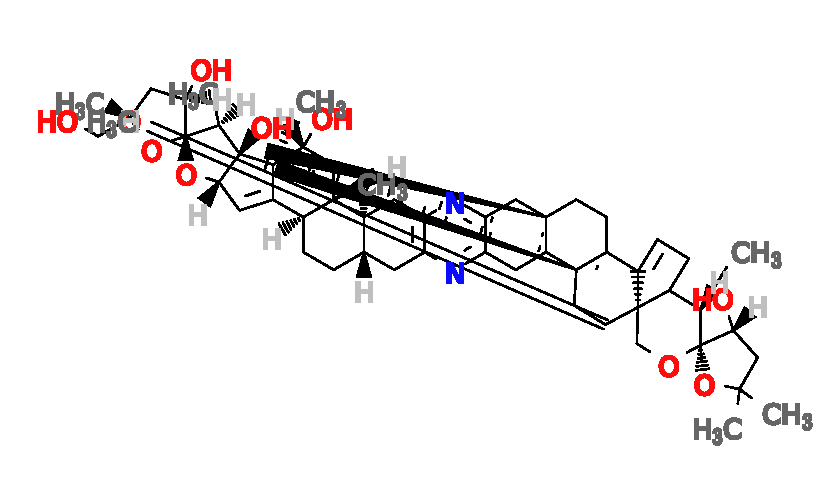
\includegraphics[scale=0.85]{figures/Mac231-Cephalostatin-1.pdf}
  \caption{Cephalostatin-1 (figure from Open Babel for Mac 2.3.1)}
  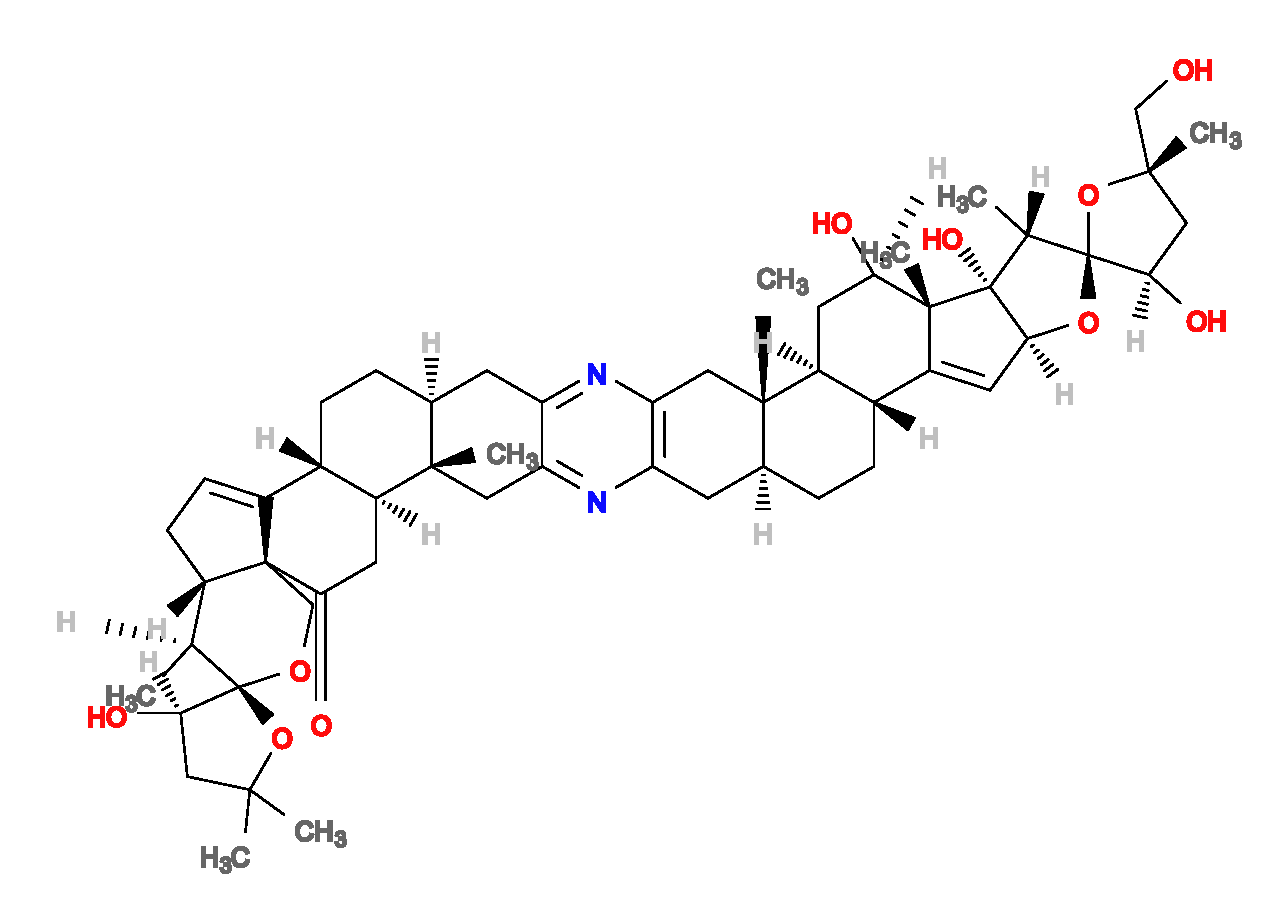
\includegraphics[scale=0.5]{figures/Win232-Cephalostatin-1.pdf}
  \caption{Cephalostatin-1 (figure from Open Babel for Win 2.3.2)}
\end{center}
\end{figure}

\begin{figure}[p]
Sesamin: \verb|c1cc2c(cc1C3C4COC(C4CO3)c5ccc6c(c5)OCO6)OCO2|
\begin{center}
  \centering
  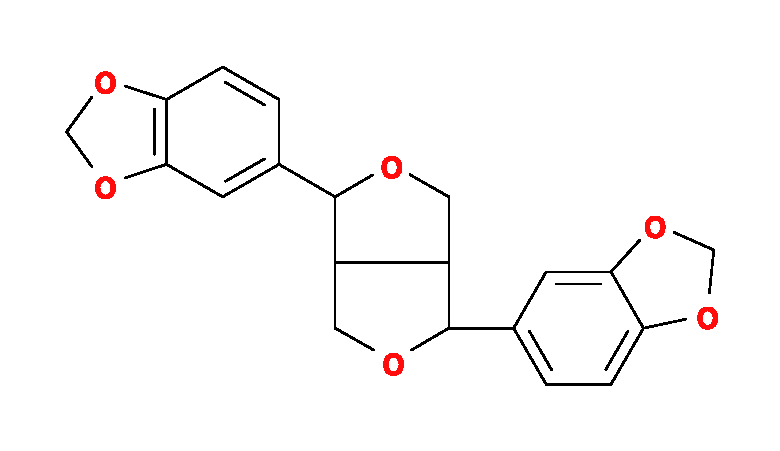
\includegraphics[scale=0.5]{figures/Mac231-sesamin-normal.pdf}
  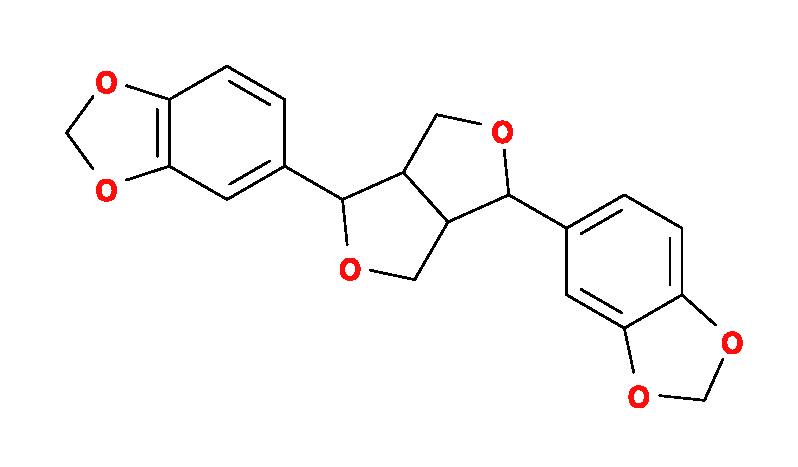
\includegraphics[scale=0.5]{figures/Mac231-sesamin-gen2d.pdf}
  \caption{Sesamin (figures from Open Babel for Mac 2.3.1; Normal and \texttt{--gen2d})}
  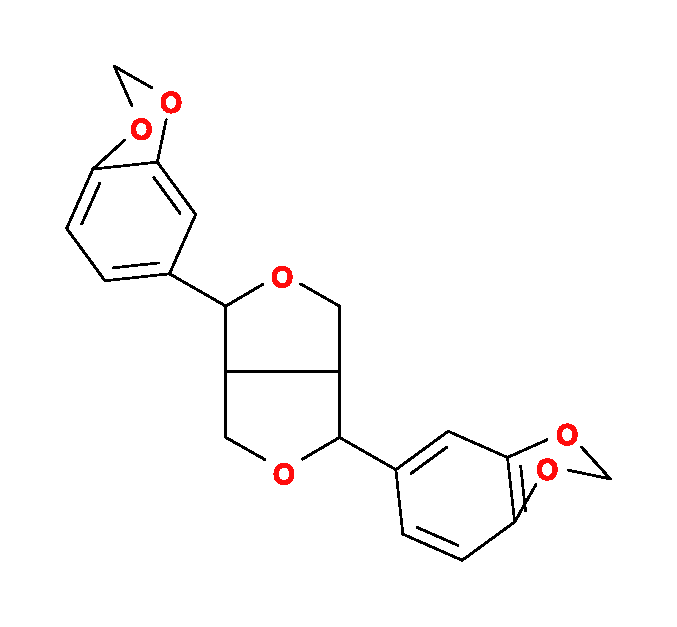
\includegraphics[scale=0.5]{figures/Win232-sesamin-normal.pdf}
  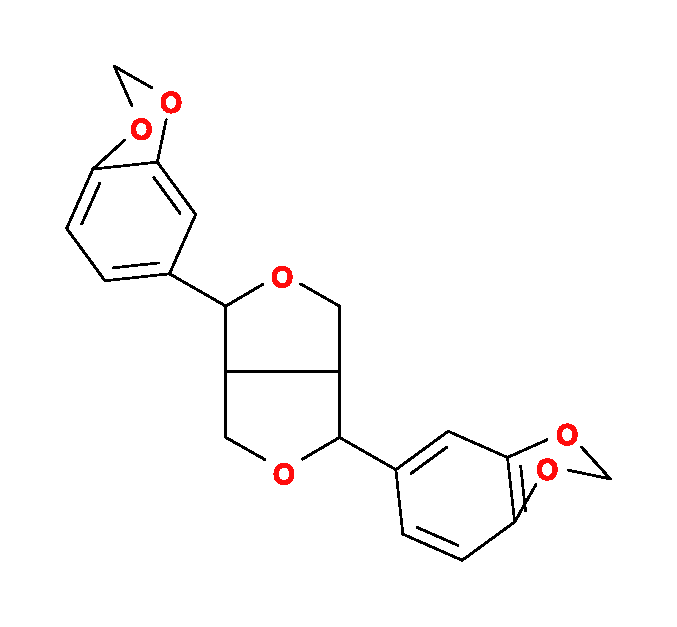
\includegraphics[scale=0.5]{figures/Win232-sesamin-gen2d.pdf}
  \caption{Sesamin (figures from Open Babel for Win 2.3.2; Normal and \texttt{--gen2d})}
\end{center}
\end{figure}

\clearpage

Also, Open Babel can generate wrong structures from SMILES notations.
Here we can see the formula generated from a SMILES notation lacks one double bond.

\begin{figure}[ht]
  \centering
  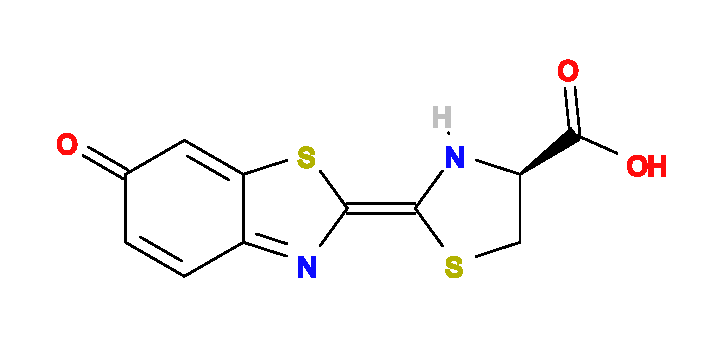
\includegraphics[scale=0.6]{figures/Exact-FireflyLuciferin.pdf}
  \caption{Firefly luciferin: exact structure from ChemSpider ID 4588411}
  \begingroup
    \catcode`\~=0
    \catcode`\%=11
    \catcode`\\=11
    ~smilesobabel[scale=0.6]{C1[C@@H](N/C(=c\2/nc3c(=CC(=O)C=C3)s2)/S1)C(=O)O}{}
  ~endgroup
%  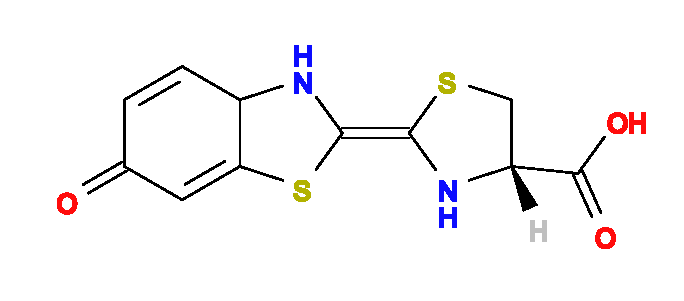
\includegraphics[scale=0.6]{Win232-FireflyLuciferin.pdf}
  \caption{Firefly luciferin?: output from Open Babel for Win 2.3.2}
  SMILES: \verb|C1[C@@H](N/C(=c\2/nc3c(=CC(=O)C=C3)s2)/S1)C(=O)O|
\end{figure}

We can avoid all these problems by using \verb|\chemobabel| with \verb|.mol| or \verb|.cdx| files, instead of \verb|\smilesobabel|.
However, the fact that many complex structures can be generated from only one character string is very interesting, isn't it?

\subsection{日本語}

図はすべて英語版を参照してください。 \\

Open Babel は SMILES 表記から複雑な構造式を生成することができます。

しかし、時には結果が望ましくないことがあり、また使用するバージョン番号によって出力が異なることがあります。
いくつかの例を示します: \\

また、Open Babel は SMILES 表記から誤った構造式を生成することもあります。
ホタルルシフェリンの図で、SMILES 表記から生成した構造式には二重結合が一つ欠けています。

このような問題点は全て \verb|.mol| または \verb|.cdx| を用意して \verb|\chemobabel| を利用することで回避できます。
とはいえ、ただの文字列から複雑な構造式を生成しうるということ自体、おもしろいとは思いませんか?

\section{Limitations and Alternatives (この方法の限界と代替案)}

\subsection{English}

This method relies on Open Babel for generating structural formulas, even without drawing anything by yourself.
Of course you can modify and customize these structures to some extent, but this method will not be suitable for fine control of the output.
Also, computer-generated formulas may sometimes be unnatural and undesirable.
Therefore this method will be useful only when you need a simple method for inserting structural formulas with minimal modification.
If you are not satisfied with the output, consider using {\XyMTeX} or \textsf{chemfig} packages instead.

I also found following packages which can be used for similar purpose:
\begin{itemize}
\item \href{http://www.ctan.org/pkg/mol2chemfig}{\textsf{mol2chemfig}}: convert chemical structures from MDL molfile format to \textsf{chemfig} source code
\end{itemize}

\subsection{日本語}

この方法は Open Babel に依存して構造式を生成しており、一切自分で構造式を描画することなく済ませることさえ可能です。
もちろんある程度はそれらの構造を修正したりカスタマイズしたりできますが、この方法は出力の緻密な調節には不向きでしょう。
また、コンピュータによって生成される構造式は時に見た目が不自然で、好ましくない場合もあるかもしれません。
したがって、この方法は構造式の出力を完全に制御したいという意図がなく、構造式を簡便に挿入したい場合にのみ。
出力に満足できない場合は、\XyMTeX や \textsf{chemfig} のようなパッケージを代わりに使うことをご検討ください。

同様の目的を達成するために使えそうなパッケージとして、以下のようなものもあります:
\begin{itemize}
\item \href{http://www.ctan.org/pkg/mol2chemfig}{\textsf{mol2chemfig}}: convert chemical structures from MDL molfile format to \textsf{chemfig} source code
\end{itemize}

\clearpage

\section{Technical information (技術情報)} \label{detail}

I read online \href{http://www.daylight.com/meetings/summerschool98/course/dave/smiles-intro.html}{SMILES Tutorial}, and checked what kinds of characters are used in SMILES syntax.
\begin{itemize}
\item Roman alphabets: \verb|A-Z|, \verb|a-z|
\item Numbers: \verb|1-10|
\item Brackets: \verb|[ ] ( )|
\item Others:
\begin{itemize}
\item \verb|*| (unspecified atomic number)
\item \verb|.| (disconnection)
\item \verb|+| (charge sign)
\item \verb|-| (single bond or charge sign)
\item \verb|=| (double bond)
\item \verb|#| (triple bond)
\item \verb|$| (quadruple bond)
\item \verb|:| (aromatic bond)
\item \verb|%| (used when more than 10 ring closures)
\item \verb|/|, \verb|\| (configuration around double bonds)
\item \verb|@| (tetrahedral chirality)
\item \verb|>| (reaction)
\end{itemize}
\end{itemize}

It is important to prevent these characters from being translated as {\LaTeX} control sequence.
However, a backslash (\verb|\|) is a default escape character in {\LaTeX}, and a percent symbol (\verb|%|) also has a special meaning as a comment character.
To solve this problem, I chose a tilde (\verb|~|) to work as an escape character in replace of a backslash by changing category codes. \\

本パッケージを制作するにあたり、オンラインの \href{http://www.daylight.com/meetings/summerschool98/course/dave/smiles-intro.html}{SMILES Tutorial}を読んで SMILES 表記法に用いられる文字の種類を調べました(一覧は英語部分参照)。

これらの文字が \LaTeX におけるコントロールシーケンスとして解釈されることを防ぐ必要がありますが、バックスラッシュ \verb|\| はデフォルトのエスケープ文字であり、またパーセント記号 \verb|%| もコメント文字としての特殊な意味を持っています。
この問題を回避するため、今回カテゴリーコードを変更することで「チルダ \verb|~|」をバックスラッシュの代わりにエスケープ文字として用いるようにしました。

\clearpage

To do (if possible):
\begin{itemize}
\item Check whether \texttt{obabel} and \texttt{inkscape} are successfully installed or not, before running programs.
\item The method for changing category codes is not sophisticated (users have to change them on their own!), so further improvement needed.
\end{itemize}

\section{Version History}

\begin{table}[h]
\centering
\begin{tabular}{rll}
Version 0.1 (December 1, 2014): & Made public (as \textsf{smilesobabel.sty}) \\
Version 0.2 (December 2, 2014): & Add options which can be passed to obabel. \\
Version 0.3 (December 7, 2014): & Change name of package: \textsf{chemobabel.sty} \\
 & Images are stored in \texttt{chemobabelimgdir}. \\
 & Add \verb|\chemobabel| command. \\
Version 0.4 (December 9, 2014): & Fix a bug: (Thanks: Yusuke Terada) \\
 & Extra spaces at the end of lines are removed. \\
Version 0.5 (December 20, 2014): & Add an option: \\
 & \verb|extract| option can load the macro easily.
\end{tabular}
\end{table}

\textbf{Important!}
\begin{itemize}
\item In Version 0.2, the number of parameters set in \verb|\smilesobabel| is changed!
\item From Version 0.3, the package name is changed to \textsf{chemobabel.sty}.
\end{itemize}

\clearpage

\begin{thebibliography}{9}
\bibitem{NOB1}
\href{http://baoilleach.blogspot.jp/2012/03/cheer-up-your-latex-with-smiles-support.html}{Cheer up your {\LaTeX} with SMILES support} -- Noel O'Blog
\bibitem{NOB2}
\href{http://baoilleach.blogspot.jp/2012/04/cheer-up-your-latex-with-smiles-support.html}{Cheer up your {\LaTeX} with SMILES support II} -- Noel O'Blog
\bibitem{JLA}
\href{http://imada.sdu.dk/~jlandersen/}{{\LaTeX}: Graphviz and OpenBabel} -- Jakob Lykke Andersen
\bibitem{OKU}
\href{http://oku.edu.mie-u.ac.jp/tex/mod/forum/discuss.php?d=1411}{文章内の画像のみを表示する方法} -- {\TeX} Forum \\
(How to extract only figures in {\LaTeX} source)
\bibitem{ACE1}
\href{http://acetaminophen.hatenablog.com/entry/2014/11/02/130624}{化学構造式を \TeX で(1):自動化による簡単生成} -- Acetaminophen's diary \\
(Chemical Structural Formula in {\LaTeX} (1): An Easy Method by Auto-generation)
\bibitem{ACE2}
\href{http://acetaminophen.hatenablog.com/entry/2014/11/02/130624}{化学構造式を \TeX で(2):自動化の注意点と解消法} -- Acetaminophen's diary \\
(Chemical Structural Formula in {\LaTeX} (2): Important Notes for Auto-generation and Solution)
\bibitem{ACE3}
\href{http://acetaminophen.hatenablog.com/entry/2014/11/05/135927}{化学構造式を \TeX で(3):補足事項} -- Acetaminophen's diary \\
(Chemical Structural Formula in {\LaTeX} (3): Supplement)
\end{thebibliography}

\noindent
\textbf{Note}: \href{http://acetaminophen.hatenablog.com/}{Acetaminophen's diary} is my own blog! (Sorry, but only in Japanese)

I added a post about this package on the 8th day of \href{http://www.adventar.org/calendars/553}{{\TeX} \& {\LaTeX} Advent Calendar 2014} (in Japanese):
\begin{itemize}
\item \href{http://acetaminophen.hatenablog.com/entry/2014/12/08/053519}{誰でも簡単! 化学構造式を \LaTeX に取り込むパッケージ} -- Acetaminophen's diary \\
(An easy way to insert chemical structural formulas into {\LaTeX} documents)
\end{itemize}

\end{document}